\documentclass[11pt,a4]{jarticle}
\usepackage[top=25truemm,bottom=30truemm,left=20truemm,right=20truemm]{geometry}
\usepackage{graphicx}
\usepackage{comment}
\begin{document}

%\tableofcontents

\section{実験手法}
\subsection{磁性体のシミュレーション}
2次元イジングモデルを用いて磁性体のシミュレーションを行った。
磁性体の結晶は単位胞を上下に32個、左右に32個それぞれ並べて、周期的境界条件を課した2次元のトーラスでモデル化した。本実験では特に断らない限り、正方格子を単位胞にもつと仮定した。
ボルツマン係数$k_B=1$となる単位系を用いた。

イジングモデルの全体のエネルギーは、格子上のスピンを$s_i$ , 磁場の強さをHとして、以下で与えられる。右辺第一項は隣接したサイト間の相互作用エネルギーを意味する。
\begin{equation}
E = -J \sum_{隣接} s_i s_j -  H \sum_{i} s_i 
\end{equation}

\subsubsection{自発磁化の温度変化}
磁場を印加しない条件で、自発磁化(磁場を印加しない条件で現れる磁化)を以下のように調べた。
まず交換相互作用の強さ$J$を1と−1の二通りの値に設定し、それぞれの場合について温度を下げていったときの自発磁化の振る舞いを調べた。
次に交換相互作用の強さ$J$を0.5で固定し、常磁性相と強磁性相を転移する温度(転移温度)を調べ、転移温度付近で自発磁化の振る舞いを調べた。転移温度は正方格子モデルと蜂の巣状格子モデルともに算出した。
さらに、高温で自発磁化がどう振る舞うか調べた。

\subsubsection{磁化曲線}
印加した磁場Hに対する平均磁化Mの振る舞い(磁化曲線)を調べた。このときの交換相互作用の値Jは1に固定し、温度は0.5に設定した。さらに人為的にスピン配置に変更を加えることで、印加した磁場に対する磁化の振る舞いがどう変わるかを定性的に調べた。

\subsubsection{磁化率と磁化のゆらぎ}

磁化率は、磁界Hに対する磁化Mの応答により定義される(式\ref{eq:chi1})。
\begin{equation}
\chi = \frac{1}{N} \frac{\partial M}{\partial H}
  \label{eq:chi1}
\end{equation}

また磁化率は、磁場を印加しない条件での磁化のゆらぎ(分散)を用いて関係\ref{eq:chi2}から計算できる。
\begin{equation}
\chi = \frac{ <M^2> - <M>^2}{N T}
  \label{eq:chi2}
\end{equation}

相互作用の強さJ=0.5の条件で、磁化率を二通りの方法(式\ref{eq:chi1}、\ref{eq:chi2})で計算し、それらの計算が一致することを確かめた。つぎに磁化率の温度依存性を磁化のゆらぎから計算し(式\ref{eq:chi2})、その転移温度付近での振る舞いを調べた。

\section{実験結果}
\subsection{磁性体のシミュレーション}
%イジングモデル、相転移

\subsubsection{自発磁化の温度変化}
交換相互作用の強さJ=1かつ温度T=1の条件での、スピン配置を図\ref{fig:positiveJ_config}に示した。
十分に低い温度(T=1)でスピン全体の向きが揃い、強磁性状態が現れることが見て取れる。
このときの平均磁化の時間変化を図\ref{fig:positiveJ_transition}に示した。
平均磁化M=0のランダムな初期スピン配置から、全体のスピンが揃い平均磁化の絶対値が大きくなっていく様子が見てとれる。
\begin{figure}[htbp]
 \begin{minipage}{0.45\hsize}
  \begin{center}
   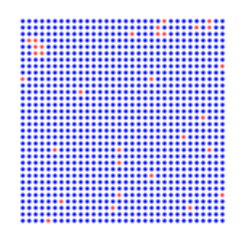
\includegraphics[width=0.9\hsize]{positiveJ_config.eps}
  \end{center}
  \caption{スピン配置(J=1; T=1)}
  \label{fig:positiveJ_config}
 \end{minipage}
 \begin{minipage}{0.55\hsize}
  \begin{center}
   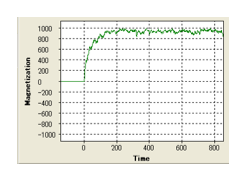
\includegraphics[width=0.9\hsize]{positiveJ_transition.eps}
  \end{center}
  \caption{磁化の時間変化(J=1; T=1)}
  \label{fig:positiveJ_transition}
 \end{minipage}
\end{figure}


交換相互作用の強さJ=-1かつ温度T=1の条件での、スピン配置を図\ref{fig:negativeJ_config}に示した。
十分に低い温度(T=1)で隣接したスピンが互いに反対向き(市松模様)になり、反磁性状態が現れる様子が見て取れる。
このときの平均磁化の時間変化を図\ref{fig:negativeJ_transition}に示した。
平均磁化M=0のランダムな初期スピン配置から、平均磁化は0のまま変化しなかった。
\begin{figure}[htbp]
 \begin{minipage}{0.45\hsize}
  \begin{center}
   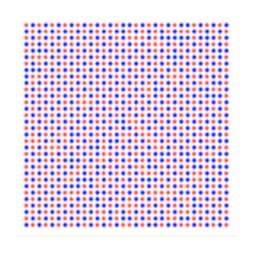
\includegraphics[width=0.9\hsize]{negativeJ_config.eps}
  \end{center}
  \caption{スピン配置(J=-1; T=1)}
  \label{fig:negativeJ_config}
 \end{minipage}
 \begin{minipage}{0.55\hsize}
  \begin{center}
   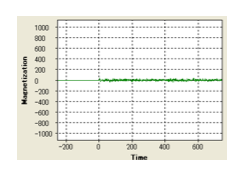
\includegraphics[width=0.9\hsize]{negativeJ_transition.eps}
  \end{center}
  \caption{磁化の時間変化(J=-1; T=1)}
  \label{fig:negativeJ_transition}
 \end{minipage}
\end{figure}


次に交換相互作用の強さJ=0.5の条件で正方格子モデル、蜂の巣状格子モデルそれぞれの転移温度Tcを調べ、表\ref{tab:Tc}に示した。また正方格子モデルの転移温度(T=0.56)でのスピン配置を図\ref{fig:criticalT_config}に示した。転移温度周辺でスピンは島のように部分的にまとまった配置になることが分かった。そのときの平均磁化の時間変化を図\ref{fig:criticalT_transition}に示した。平均磁化は時間とともに大きく揺らぐことが分かった。
\begin{table}[htbp]
   \begin{center}
  \begin{tabular}{ccc}
    正方格子 & 蜂の巣格子\\ \hline
    0.56 & 0.40\\
  \end{tabular}
  \label{tab:Tc}
     \end{center}
       \caption{転移温度}
\end{table}
\begin{figure}[htbp]
 \begin{minipage}{0.45\hsize}
  \begin{center}
   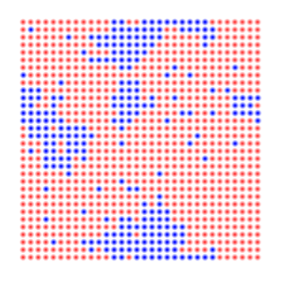
\includegraphics[width=0.9\hsize]{criticalT_config.eps}
  \end{center}
  \caption{転移温度($Tc=0.56$)付近でのスピン配置}
  \label{fig:criticalT_config}
 \end{minipage}
 \begin{minipage}{0.55\hsize}
  \begin{center}
   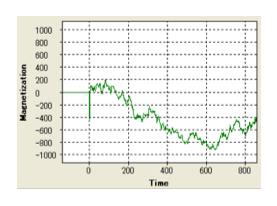
\includegraphics[width=0.9\hsize]{criticalT_transition.eps}
  \end{center}
  \caption{転移温度($Tc=0.56$)付近での磁化の時間変化}
  \label{fig:criticalT_transition}
 \end{minipage}
\end{figure}


温度Tが転移温度に比べて十分に大きい条件(T=1.5)での、スピン配置を図\ref{fig:HighT_config}に示した。
高温でスピンがランダムに並び、常磁性状態が現れる様子が見て取れる。
このときの平均磁化の時間変化を図\ref{fig:negativeJ_transition}に示した。
平均磁化M=0のランダムな初期スピン配置から、平均磁化は0のまま変化しなかった。
\begin{figure}[htbp]
 \begin{minipage}{0.45\hsize}
  \begin{center}
   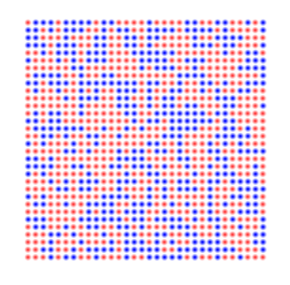
\includegraphics[width=0.9\hsize]{HighT_config.eps}
  \end{center}
  \caption{転移温度以上でのスピン配置(T=1.5)}
  \label{fig:HighT_config}
 \end{minipage}
 \begin{minipage}{0.55\hsize}
  \begin{center}
   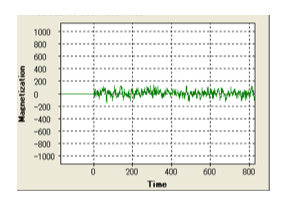
\includegraphics[width=0.9\hsize]{HighT_transition.eps}
  \end{center}
  \caption{転移温度以上での磁化の時間変化(T=1.5)}
  \label{fig:HighT_transition}
 \end{minipage}
\end{figure}

\subsubsection{磁化曲線}
相互作用の強さJ=1かつ温度T=0.5の条件での磁化曲線を、図\ref{fig:Ferromagnetism}に示した。磁場Hを-0.5から0.5まで断熱的に変化させると、磁場H=0.28程度で磁化Mが-1024程度から1024程度に一気に反転した。ここで$0<H<0.28$の条件では磁界と磁化の向きは反対向きである。Hが0.28を超えると磁化が一気に反転して磁化と磁界は同じ方向を向く。このときの磁界の強さ(の絶対値)を反転磁場と呼ぶ。
またHを0.5から-0.5に断熱変化させると、H=-0.28程度でMが一気に反転した。
\begin{figure}[htbp]
  \begin{center}
   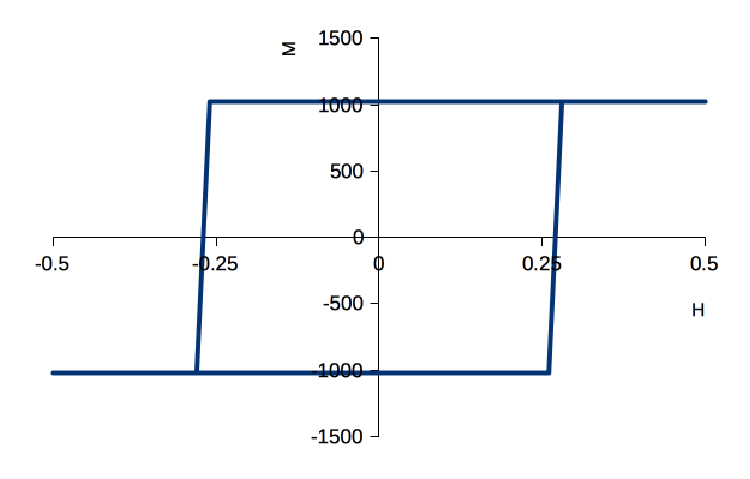
\includegraphics[width=0.75\hsize]{Ferromagnetism.eps}
  \end{center}
  \caption{強磁性体の磁化曲線(J=1; T=0.5)}
  \label{fig:Ferromagnetism}
\end{figure}

次にH=-0.5から0.25まで磁界を変化させてH=0.25で固定し、いくつかのスピンを人為的に反転させたとき(反転させたスピンを核と呼ぶ)、反転磁場以下の磁場でも磁化の反転が確認できた。
要素が16個未満の核で磁化の反転は確認できず、要素が16個以上の核でも形が細長いと磁化の反転が引き起こされないことが確認できた。磁化の反転を引き起こす核は、要素を少なくとも16個持ち、正方形に近くなければならない。すなわち、磁化の反転は核の要素数と形状に依存することが分かった

\subsubsection{磁化率と磁化のゆらぎ}
J=0.5の条件で、磁化率を二通りの方法(式\ref{eq:chi1},\ref{eq:chi2})で計算し、温度に対してプロットしたものを図\ref{fig:comparison_chi}に示した。ここでオレンジ色のマーカーで示したデータが式\ref{eq:chi1}、青色が式\ref{eq:chi2}に対応している。
相対誤差は高々15$\%$程度であり、よい精度での一致が見られた。
\begin{figure}[htbp]
  \begin{center}
   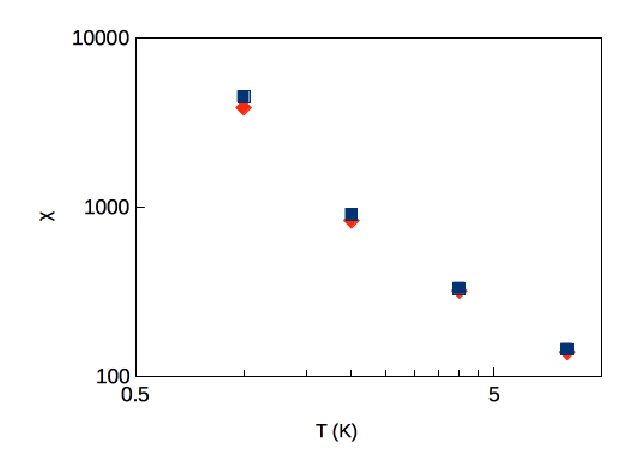
\includegraphics[width=0.75\hsize]{comparison_chi.eps}
  \end{center}
  \caption{異なる方法で求めた磁化率の比較}
  \label{fig:comparison_chi}
\end{figure}

式\ref{eq:chi2}を用いて磁化のゆらぎから計算した磁化率の温度依存性を、図\ref{fig:temperature_dependence_chi}に両対数プロットした。磁化率はT=0.65付近で特異的に大きい。T=0.65を転移温度とすると、臨界定数は-1.06と見積もれた。
\begin{figure}[htbp]
  \begin{center}
   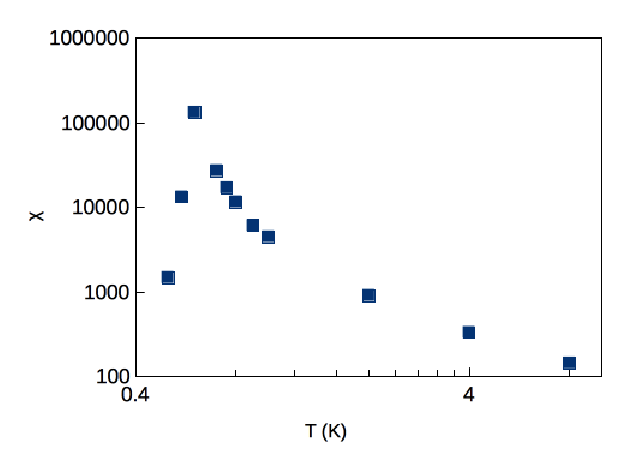
\includegraphics[width=0.75\hsize]{temperature_dependence_chi.eps}
  \end{center}
  \caption{磁化率の温度依存性}
  \label{fig:temperature_dependence_chi}
\end{figure}

\section{考察}
\subsection{磁性体のシミュレーション}
\subsubsection{自発磁化の温度変化}
まず正方格子モデルに関して、自発磁化の温度依存性を考察する。

$J>0$のとき: 
転移温度に比べて系の温度が十分に低いとき、自発磁化が現れることが分かった。このとき全体のスピンの向きが揃っていた。これは$J>0$の条件で、全体のスピンが揃っていたほうがサイト間の相互作用エネルギーが小さくなることから説明できる。
転移温度に比べて系の温度が十分に高いとき、自発磁化は現れず、スピンの向きはランダムになった。これはエネルギーの熱的な励起の影響である。
転移温度付近で磁化は大きく揺らぎ、そのときスピンは島状の配置になった。熱的なエネルギー励起の影響を受けながら、系の相互作用エネルギーを小さくしようとする系の性質を反映した振る舞いである、と筆者は考える。

$J<0$のとき: 自発磁化は現れなかった。

次に正方格子モデルと蜂の巣状格子モデルの転移温度Tcに関して考察する。
転移温度Tcを実験で求めたところ、正方格子モデルと蜂sの巣状格子モデルはそれぞれ0.56と0.40であった。
対して、2次元Isingモデルの転移温度Tcは解析解が得られており、それぞれ$J/ln(1+\sqrt{2})=0.567$と$J/ln(2+\sqrt{3})=0.380$である。
実験値と解析値の間には高い精度の一致が見られる。

正方格子モデルと蜂の巣状格子モデルの間の転移温度の違いは、隣接サイト数の違いに起因する。
正方格子モデルでそれぞれのサイトに隣接するサイトは4つ存在するが、蜂の巣状格子モデルでは3つである。これから蜂の巣状格子モデルに比較すると正方格子モデルでは相互作用エネルギーの影響が大きく、それを熱的な励起で相殺するための温度、すなわち転移温度が大きくなる。


\subsubsection{磁化曲線}
強磁性状態で磁化と磁界が逆向きのとき、核が磁化の反転を引き起こすかどうかはその要素数と形状に依存する。これは周りとのサイト間の相互作用エネルギー$E_{int}$と、磁場とスピンの相互作用エネルギー$E_{mag}$を考えれば理解できる。核が存在すると、$E_{int}$は大きくなり、$E_{mag}$は小さくなる。
$E_{mag}$は核の要素数に比例するが、それに比べて$E_{int}$の影響は核の要素数が小さければ大きくなる。ここから核の要素が少なすぎると全体のエネルギーが高くなってしまうことが分かる。また$E_{int}$は細長い形で大きくなるので、丸っこい形がエネルギーを考えたときに有利である。したがって、磁化の反転を引き起こす核は要素を一定数以上持つことが必要で、正方形状に近い方が有利である。

\subsubsection{磁化率と磁化のゆらぎ}
実験で求めた臨界係数-1.06を、理論により計算した臨界係数-1.75と比較すると、誤差の範囲内で一致しない。この実験値と解析値の差は、系の転移温度を精度よく見積もれなかったことや、実験系の大きさが有限であることに起因すると筆者は考える。

\end{document}


